\subsection{Model}
\label{sec:Model}

\begin{figure}[ht]
\begin{center}
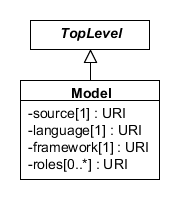
\includegraphics[scale=0.6]{uml/model}
\caption[]{Diagram of the \sbol{Model} class and its associated properties.}
\label{uml:model}
\end{center}
\end{figure}

The purpose of the \sbol{Model} class is to serve as a placeholder for an external computational model and provide additional meta-data to enable better reasoning about the contents of this model.
In this way, there is minimal duplication of standardization efforts and users of SBOL can formalize the function of a \sbol{Component} in the language of their choice.

The meta-data provided by the \sbol{Model} class include the following properties: the \sbolmult{source:M}{source} or location of the actual content of the model, the \sbol{language} in which the model is implemented, and the model's \sbol{framework}.

\subparagraph{ The \sbolheading{source} property}\label{sec:source:M}
The \sbolmult{source:M}{source} property is REQUIRED and MUST contain a \sbol{URI} reference to the source file for a model.

\subparagraph{ The \sbolheading{language} property}\label{sec:language}
The \sbol{language} property is REQUIRED and MUST contain a \sbol{URI} that specifies the language in which the model is implemented. It is RECOMMENDED that this \sbol{URI} refer to a term from the EMBRACE Data and Methods (EDAM) ontology. \ref{tbl:model_types} provides a list of terms from this ontology and their \sbol{URI}s. If the \sbol{language} property of a \sbol{Model} is well-described by one these terms, then it MUST contain the \sbol{URI} for this term as its value.

\begin{table}[ht]
  \begin{edtable}{tabular}{ll}
    \toprule
    \textbf{Model Language} & \textbf{URI for EDAM Term} \\
    \midrule
    SBML  & \url{http://identifiers.org/edam/format_2585}\\
    CellML		 & \url{http://identifiers.org/edam/format_3240}\\
    BioPAX    & \url{http://identifiers.org/edam/format_3156}\\
    \bottomrule
  \end{edtable}
  \caption{Terms from the EDAM ontology to specify the \sbol{language} property of a \sbol{Model}.}
  \label{tbl:model_types}
\end{table}


\subparagraph{ The \sbolheading{framework} property}\label{sec:framework}
The \sbol{framework} property is REQUIRED and MUST contain a \sbol{URI} that specifies the framework in which the model is implemented.
It is RECOMMENDED this \sbol{URI} refer to a term from the modeling framework branch of the SBO when possible. A few suggested modeling frameworks and their corresponding \sbol{URI}s are shown in \ref{tbl:model_frameworks}. If the \sbol{framework} property of a \sbol{Model} is well-described by one these terms, then it MUST contain the \sbol{URI} for this term as its value.

\begin{table}[ht]
  \begin{edtable}{tabular}{ll}
    \toprule
    \textbf{Framework} & \textbf{URI for SBO Term} \\
    \midrule
    Continuous  & \url{http://identifiers.org/biomodels.sbo/SBO:0000062}\\
    Discrete & \url{http://identifiers.org/biomodels.sbo/SBO:0000063}\\
    \bottomrule
  \end{edtable}
  \caption{SBO terms to specify the \sbol{framework} property of a \sbol{Model}.}
  \label{tbl:model_frameworks}
\end{table}
